
\documentclass[a4paper,11pt]{article}

% Math symbols
\usepackage{amsmath}
\usepackage{amsfonts}
\usepackage{esvect}
\usepackage{mhchem}
\usepackage{chemfig}

% Hyperlink contents page
\usepackage{hyperref}
\hypersetup{
	colorlinks,
	citecolor=black,
	filecolor=black,
	linkcolor=black,
	urlcolor=black
}

% No indent on new paragraphs
\setlength{\parindent}{0mm}
\setlength{\parskip}{0.2cm}

% AI files
\usepackage{graphicx}
\DeclareGraphicsRule{.ai}{pdf}{.ai}{}

% Style for organic diagrams
\setdoublesep{0.35700 em}
\setatomsep{1.78500 em}
\setbondoffset{0.18265 em}
\newcommand{\bondwidth}{0.06642 em}
\setbondstyle{line width = \bondwidth}

% For Polymer braces
\newcommand\setpolymerdelim[2]{\def\delimleft{#1}\def\delimright{#2}}

\def\makebraces(#1,#2)#3#4#5{%
  \edef\delimhalfdim{\the\dimexpr(#1+#2)/2}%
  \edef\delimvshift{\the\dimexpr(#1-#2)/2}%
  \chemmove{
    \node[at=(#4),yshift=(\delimvshift)]
      {$
       \left\delimleft
         \vrule height\delimhalfdim depth\delimhalfdim width0pt
       \right.
      $};
    \node[at=(#5),yshift=(\delimvshift)]
      {$
        \left.
          \vrule height\delimhalfdim depth\delimhalfdim width0pt
        \right\delimright_{\rlap{#3}}
      $};
  }%
}

\setpolymerdelim()


\begin{document}

\title{Organic}
\author{Ben Anderson}
\date{\today}
\maketitle
\pagebreak

\tableofcontents
\pagebreak


\section{Organic Molecules}

A molecule that contains only non-metal elements, and at least one carbon.

\subsection{Chain Length}

Carbon chain length prefixes:

\begin{enumerate}
\item meth-
\item eth-
\item prop-
\item but-
\item pent-
\item hex-
\item hept-
\item oct-
\item non-
\item dec-
\end{enumerate}




\section{Alkanes}

Suffix: -an

Only contain Carbon/Carbon single bonds.

Formula: $\ce{C_{n}H_{2n + 2}}$


\subsection{Examples}

Methane ($\ce{CH4}$):

\begin{center}
\chemfig{C(-[::0]H)(-[::90]H)(-[::180]H)(-[::270]H)}
\end{center}

Butane ($\ce{CH3CH2CH2CH3}$):

\begin{center}
\chemfig{C(-[::0]C(-[::0]C(-[::0]C(-[::0]H)(-[::90]H)(-[::270]H))(-[::90]H)(-[::270]H))(-[::90]H)(-[::270]H))(-[::90]H)(-[::180]H)(-[::270]H)}
\end{center}


\subsection{Substitution Reaction}

Reaction between an alkane and a halogen.

Replaces a Hydrogen off a Carbon on the alkane.

Produces the hydride of the halogen.

A slow reaction, sped up in the presence of UV light.


\subsubsection{Multiple Substitutions}

Multiple Hydrogen atoms can be substituted for the halogen on the same molecule.

\begin{description}
\item [Monosubstitution] Replacement of 1 Hydrogen atom
\item [Disubstitution] Replacement of 2 Hydrogen atoms
\item [Trisubstitution] ...
\end{description}


\subsubsection{Examples}

Methane and chlorine mono-substitution:

\begin{center}
\ce{\chemfig{C(-[::0]H)(-[::90]H)(-[::180]H)(-[::270]H)} + Cl2 ->
	\chemfig{C(-[::0]H)(-[::90]Cl)(-[::180]H)(-[::270]H)} + HCl}
\end{center}

Methane and chlorine di-substitution:

\begin{center}
\ce{\chemfig{C(-[::0]H)(-[::90]Cl)(-[::180]H)(-[::270]H)} + Cl2 ->
	\chemfig{C(-[::0]Cl)(-[::90]Cl)(-[::180]H)(-[::270]H)} + HCl}
\end{center}




\section{Alkenes}

Suffix: -en

Contain at least 1 Carbon/Carbon double bond.

Formula (for 1 double bond): $\ce{C_{n}H_{2n}}$

Methene doesn't exist.


\subsection{Naming}

Position of double bond included in name.

Carbon atoms are numbered in sequence to minimise the number assigned to the
double bond.


\subsection{Examples}

Ethene ($\ce{CH2CH2}$):

\begin{center}
\chemfig{C(=[::0]C(-[::45]H)(-[::-45]H))(-[::135]H)(-[::-135]H)}
\end{center}

Propene ($\ce{CH2CHCH3}$):

\begin{center}
\chemfig{C(=[::0]C(-[::45]C(-[::0]H)(-[::90]H)(-[::270]H))(-[::-45]H))(-[::135]H)(-[::-135]H)}
\end{center}

But-1-ene ($\ce{CH2CHCH2CH3}$):

\begin{center}
\chemfig{C(=[::0]C(-[::45]C(-[::0]C(-[::0]H)(-[::90]H)(-[::270]H))(-[::90]H)(-[::270]H))(-[::-45]H))(-[::135]H)(-[::-135]H)}
\end{center}


\subsection{Addition Reaction}

Reaction between an alkene and a halogen.

Replaces the double bond with a single bond, adding a halogen to each Carbon.

Fast reaction, no UV light needed.


\subsubsection{Examples}

Ethene and chlorine:

\begin{center}
\ce{\chemfig{C(=[::0]C(-[::45]H)(-[::-45]H))(-[::135]H)(-[::-135]H)} + Cl2 ->
	\chemfig{C(-[::0]C(-[::0]H)(-[::90]Cl)(-[::270]H))(-[::90]Cl)(-[::180]H)(-[::270]H)}}
\end{center}

But-1-ene and bromine:

\begin{center}
\ce{\chemfig{C(=[::0]C(-[::45]C(-[::0]C(-[::0]H)(-[::90]H)(-[::270]H))(-[::90]H)(-[::270]H))(-[::-45]H))(-[::135]H)(-[::-135]H)}
	+ Br2 ->
	\chemfig{C(-[::0]C(-[::0]C(-[::0]C(-[::0]H)(-[::90]H)(-[::270]H))(-[::90]H)(-[::270]H))(-[::90]Br)(-[::270]H))(-[::90]Br)(-[::180]H)(-[::270]H)}}
\end{center}


\subsection{Differentiate Between Alkene and Alkane}

Add liquid bromine (orange coloured).

Will turn colourless in an alkene due to the fast addition reaction.

Will remain orange in an alkane.




\section{Alkynes}

Suffix: -yn

Contains at least 1 Carbon/Carbon triple bond.

Position of the triple bond included in the name, like an alkene.

Methyne doesn't exist.


\subsection{Examples}

Ethyne:

\begin{center}
\chemfig{C(~[::0]C(-[::0]H))(-[::180]H)}
\end{center}

But-1-yne:

\begin{center}
\chemfig{C(~[::0]C(-[::0]C(-[::0]C(-[::0]H)(-[::90]H)(-[::270]H))(-[::90]H)(-[::270]H)))(-[::180]H)}
\end{center}




\section{Hydrocarbons}

Molecules containing only Carbon and Hydrogen.

Will combust in presence of Oxygen and a flame (activation energy).


\subsection{Complete Combustion}

$$
\ce{CH4 + 2O2 -> CO2 + H2O}
$$

Any hydrocarbon will combust in an excess of oxygen.

Will form only carbon dioxide and water.


\subsection{Partial Combustion}

$$
\ce{CH4 + O2 -> CO + H2O}
$$

Occurs when Oxygen supply is limited.

Forms leathal carbon monoxide.


\subsection{Incomplete Combustion}

$$
\ce{CH4 + O2 -> C + 2H2O}
$$

Occurs when Oxygen supply is very limited.

Forms just Carbon.




\section{Halogens}

A halogen can replace any carbon on an organic molecule.


\subsection{Naming}

The position and type of halogen are included in the name of the molecule.

The number of the carbon the halogen is attached to is used as its position.

Each halogen has an associated prefix:

\begin{center}
\begin{tabular}{c|c}
Chlorine & chloro- \\
Fluorine & fluoro- \\
Iodine   & iodo-   \\
Bromine  & bromo-  \\
\end{tabular}
\end{center}

More than 1 of the same halogen attached to the same carbon applies another
prefix specifying the number.

Minimising the number of the double bond takes precedence over any halogens.


\subsection{Examples}

Chloro methane ($\ce{CH3Cl}$):

\begin{center}
\chemfig{C(-[::0]H)(-[::90]Cl)(-[::180]H)(-[::270]H)}
\end{center}

Diiodo methane ($\ce{CH2I2}$):

\begin{center}
\chemfig{C(-[::0]I)(-[::90]I)(-[::180]H)(-[::270]H)}
\end{center}

1,2-difluoro ethane ($\ce{CH2FCH2F}$):

\begin{center}
\chemfig{C(-[::0]C(-[::0]H)(-[::90]F)(-[::270]H))(-[::90]F)(-[::180]H)(-[::270]H)}
\end{center}

4,4-dibromo 2-iodo but-1-ene ($\ce{CH2CICH2CHBr2}$):

\begin{center}
\chemfig{C(=[::0]C(-[::45]C(-[::0]C(-[::0]H)(-[::90]Br)(-[::270]Br))(-[::90]H)(-[::270]H))(-[::-45]I))(-[::135]H)(-[::-135]H)}
\end{center}



\section{Alkyl Groups}

Suffix: -yl

Side Carbon chains branching off the main Carbon chain.

Position and length of chain is included in the name.

Numbering of the double bond takes precedence over alkyl groups.


\subsection{Examples}

Methyl propane ($\ce{CH3CH(CH3)CH3}$):

\begin{center}
\chemfig{C(-[::0]C(-[::0]C(-[::0]H)(-[::90]H)(-[::270]H))(-[::90]C(-[::0]H)(-[::90]H)(-[::270]H))(-[::270]H))(-[::90]H)(-[::180]H)(-[::270]H)}
\end{center}

2-methyl butane ($\ce{CH3CH(CH3)CH2CH3}$):

\begin{center}
\chemfig{C(-[::0]C(-[::0]C(-[::0]C(-[::0]H)(-[::90]H)(-[::270]H))(-[::90]H)(-[::270]H))(-[::90,1.8]C(-[::0]H)(-[::90]H)(-[::270]H))(-[::270]H))(-[::90]H)(-[::180]H)(-[::270]H)}
\end{center}

2-ethyl butane ($\ce{CH3CH(CH2CH3)CH2CH3}$):

\begin{center}
\chemfig{C(-[::0]C(-[::0]C(-[::0]C(-[::0]H)(-[::90]H)(-[::270]H))(-[::90]H)(-[::270]H))(-[::90]C(-[::0]C(-[::0]H)(-[::90]H)(-[::270]H))(-[::90]H)(-[::270]H))(-[::270]H))(-[::90]H)(-[::180]H)(-[::270]H)}
\end{center}

2-ethyl 3-methyl pentane ($\ce{CH3CH(CH2CH3)CH(CH3)CH2CH3}$):

\begin{center}
\chemfig{C(-[::0]C(-[::0]C(-[::0]C(-[::0]H)(-[::90]H)(-[::270]H))(-[::90]H)(-[::270]H))(-[::90]H)(-[::270]H))(-[::90]H)(-[::180]H)(-[::270]H)}
\end{center}




\section{Cyclic Compounds}

Prefix: cyclo-

Where the terminal carbon is bonded to the first carbon in the chain, forming a
circle.

Formula: $\ce{C_{n}H_{2n}}$


\subsection{Examples}

Cyclobutane:

\begin{center}
\chemfig{C*4(-C(-[::0]H)(-[::270]H)-C(-[::0]H)(-[::270]H)-C(-[::0]H)(-[::270]H)-)(-[::180]H)(-[::270]H)}
\end{center}

3,4-dichloro cyclohexene:

\begin{center}
\chemfig{C*6(=C(-[::-45]H)-C(-[::-15]Cl)(-[::285]H)-C(-[::-15]Cl)(-[::285]H)-C(-[::-15]H)(-[::285]H)-C(-[::-15]H)(-[::285]H)-)(-[::180]H)(-[::270]H)}
\end{center}




\section{Isomers}

Molecules with the same molecular formula, but different arrangement of atoms.

Bonds must be broken to change one isomer into another.


\subsection{Structural Isomers}

Structural isomers have different physical sequences of atoms.


\subsubsection{Example}

$\ce{C4H10}$ could be butane:

\begin{center}
\chemfig{C(-[::0]C(-[::0]C(-[::0]C(-[::0]H)(-[::90]H)(-[::270]H))(-[::90]H)(-[::270]H))(-[::90]H)(-[::270]H))(-[::90]H)(-[::180]H)(-[::270]H)}
\end{center}

Or methyl propane:

\begin{center}
\chemfig{C(-[::0]C(-[::0]C(-[::0]H)(-[::90]H)(-[::270]H))(-[::90]C(-[::0]H)(-[::90]H)(-[::270]H))(-[::270]H))(-[::90]H)(-[::180]H)(-[::270]H)}
\end{center}


\subsection{Geometric Isomers}

No rotation can occur around a double bond.

Alkenes with different arrangements of atoms around the double bond are isomers
of each other.

Only occurs when both Carbon atoms doubly bonded together have 2 different
atoms bonded to them.


\subsubsection{Naming}

\begin{description}
\item [Cis- isomers] Where the upper or lower two atoms around the double bond
	are the same.
\item [Trans- isomers] Where the atoms across the diagonal around the double
	bond are the same.
\end{description}


\subsubsection{Examples of Geometric Isomerism}

Cis-but-2-ene:

\begin{center}
\chemfig{C(-[::-45]C(=[::45]C(-[::45]C(-[::0]H)(-[::90]H)(-[::270]H))(-[::-45]H))(-[::-90]H))(-[::-135]H)(-[::45]H)(-[::135]H)}
\end{center}

Trans-but-2-ene:

\begin{center}
\chemfig{C(-[::-45]C(=[::45]C(-[::-45]C(-[::0]H)(-[::90]H)(-[::270]H))(-[::45]H))(-[::-90]H))(-[::-135]H)(-[::45]H)(-[::135]H)}
\end{center}

1,2-dichloro trans-ethene:

\begin{center}
\chemfig{C(=[::0]C(-[::45]Cl)(-[::-45]H))(-[::135]H)(-[::-135]Cl)}
\end{center}


\subsubsection{Examples without Geometric Isomerism}

Ethene (all Hydrogens off the two Carbons):

\begin{center}
\chemfig{C(=[::0]C(-[::45]H)(-[::-45]H))(-[::135]H)(-[::-135]H)}
\end{center}

But-1-ene (two Hydrogens off the first Carbon):

\begin{center}
\chemfig{C(=[::0]C(-[::45]C(-[::0]C(-[::0]H)(-[::90]H)(-[::270]H))(-[::90]H)(-[::270]H))(-[::-45]H))(-[::135]H)(-[::-135]H)}
\end{center}

1,1-dichloro ethene:

\begin{center}
\chemfig{C(=[::0]C(-[::45]Cl)(-[::-45]Cl))(-[::135]H)(-[::-135]H)}
\end{center}




\section{Saturation}

A molecule is saturated if every Carbon has 4 atoms singly bonded to it.

No double bonds.

All alkanes are saturated.



\section{Alcohols}

Suffix: -ol

Alcohols have an $\ce{OH}$ group attached to any carbon along the main chain.

Minimising the number of the carbon with the $\ce{OH}$ group attached takes
priority over any other structure (including any double bonds).


\subsection{Properties}

Solubility decreases as carbon chain length increases:

\begin{itemize}
\item ...??
\end{itemize}

Boiling point is higher than alkanes or alkenes of similar molar mass:

\begin{itemize}
\item Alcohols experience Hydrogen bonding between molecules
\item Alkanes and alkenes experience only dispersion forces
\item For similar molar mass, Hydrogen bonding is stronger than dispersion
\item Alcohols have a higher boiling point.
\end{itemize}


\subsection{Classification}

\begin{description}
\item [Primary Alcohol] Where the Carbon the $\ce{OH}$ group is attached to
	has 0 or 1 other Carbons attached to it (eg. methanol or butan-1-ol).
\item [Secondary Alcohol] Where the Carbon the $\ce{OH}$ group is attached to
	has 2 other Carbons attached to it (eg. butan-2-ol).
\item [Tertiary Alcohol] Where the Carbon the $\ce{OH}$ group is attached to
	has 3 other Carbons attached to it (eg. methyl propan-2-ol).
\end{description}


\subsection{Isomers}

A molecular formula with an Oxygen has multiple valid structures.

For example, $\ce{C4H10O}$:

\begin{itemize}
\item Butan-1-ol
\item Butan-2-ol
\item Methyl Propan-1-ol
\item Methyl Propan-2-ol
\end{itemize}


\subsection{Examples}

Methanol ($\ce{CH3OH}$):

\begin{center}
\chemfig{C(-[::0]OH)(-[::90]H)(-[::180]H)(-[::270]H)}
\end{center}

Ethanol ($\ce{CH3CH2OH}$):

\begin{center}
\chemfig{C(-[::0]C(-[::0]OH)(-[::90]H)(-[::270]H))(-[::90]H)(-[::180]H)(-[::270]H)}
\end{center}

Ethenol ($\ce{CH2CHOH}$):

\begin{center}
\chemfig{C(=[::0]C(-[::45]OH)(-[::-45]H))(-[::135]H)(-[::-135]H)}
\end{center}

Butan-1-ol ($\ce{CH2(OH)CH2CH2CH3}$):

\begin{center}
\chemfig{C(-[::0]C(-[::0]C(-[::0]C(-[::0]H)(-[::90]H)(-[::270]H))(-[::90]H)(-[::270]H))(-[::90]H)(-[::270]H))(-[::90]OH)(-[::180]H)(-[::270]H)}
\end{center}

Butan-2-ol ($\ce{CH3CH(OH)CH2CH3}$):

\begin{center}
\chemfig{C(-[::0]C(-[::0]C(-[::0]C(-[::0]H)(-[::90]H)(-[::270]H))(-[::90]H)(-[::270]H))(-[::90]OH)(-[::270]H))(-[::90]H)(-[::180]H)(-[::270]H)}
\end{center}

Trans-but-2-en-1-ol:

\begin{center}
\chemfig{C(-[::-45]C(=[::45]C(-[::-45]C(-[::0]H)(-[::90]H)(-[::270]H))(-[::45]H))(-[::-90]H))(-[::-135]H)(-[::45]H)(-[::135]OH)}
\end{center}


\subsection{Hydration Reaction}

A reaction between an alkene and water that forms an alcohol.

Replace the double bond with a single bond.

Add $\ce{H}$ to one of the Carbons, and $\ce{OH}$ to the other.


\subsubsection{Example}

Ethene added to water:

$$
\ce{\chemfig{C(=[::0]C(-[::45]H)(-[::-45]H))(-[::135]H)(-[::-135]H)} + H2O ->
\chemfig{C(-[::0]C(-[::0]H)(-[::90]H)(-[::270]H))(-[::90]OH)(-[::180]H)(-[::270]H)}}
$$


\subsection{Redox Reaction}

Transformation of an alcohol into a different organic product.

Occurs in the presence of an acidified oxidising agent.


\subsubsection{Oxidising Agent}

Possible oxidising agents are:

\begin{itemize}
\item $\ce{H+}$ and $\ce{MnO4-}$
\item $\ce{H+}$ and $\ce{Cr2O7^2-}$
\end{itemize}

The oxidising agent will be reduced:

\begin{itemize}
\item $\ce{MnO4-}$ to $\ce{Mn^2+}$
\item $\ce{Cr2O7^2-}$ to $\ce{Cr^3+}$
\end{itemize}

The alcohol will be oxidised.


\subsubsection{Primary Alcohol}

Primary alcohol oxidises to an aldehyde.

Aldehyde oxidises to a carboxylic acid.

For example, ethanol:

\begin{center}
\chemfig{C(-[::0]C(-[::0]OH)(-[::90]H)(-[::270]H))(-[::90]H)(-[::180]H)(-[::270]H)}
\end{center}

Oxidises to ethanal:

\begin{center}
\chemfig{C(-[::0]C(=[::45]O)(-[::-45]H))(-[::90]H)(-[::180]H)(-[::270]H)}
\end{center}

Oxidises to ethanoic acid:

\begin{center}
\chemfig{C(-[::0]C(=[::45]O)(-[::-45]OH))(-[::90]H)(-[::180]H)(-[::270]H)}
\end{center}

If excess oxidising agent is added, most of the product is the carboxylic acid.

If the oxidising agent is added in stoichiometric ratios, the product is half
carboxylic acid, half aldehyde.


\subsubsection{Secondary Alcohol}

Secondary alcohol oxidises to a ketone.

For example, propan-2-ol:

\begin{center}
\chemfig{C(-[::0]C(-[::0]C(-[::0]H)(-[::90]H)(-[::270]H))(-[::90]O(-[::0]H))(-[::270]H))(-[::90]H)(-[::180]H)(-[::270]H)}
\end{center}

Oxidises to propanone:

\begin{center}
\chemfig{C(-[::0]C(-[::0]C(-[::0]H)(-[::90]H)(-[::270]H))(=[::90]O))(-[::90]H)(-[::180]H)(-[::270]H)}
\end{center}


\subsubsection{Tertiary Alcohol}

Tertiary alcohols do not undergo oxidation reactions.


\subsection{Differentiation of Alcohols}

Add an oxidising agent.

Will change colour if a primary or secondary alcohol (oxidises).

Method 1:

\begin{itemize}
\item Add calcium carbonate.
\item The primary alcohol will fizz and produce a colourless, odourless gas
	(reaction with carboxylic acid).
\end{itemize}

Method 2:

\begin{itemize}
\item Heat each solution.
\item The carboxylic acid will have a higher boiling point than the ketone due
	to Hydrogen bonding.
\end{itemize}




\section{Other Functional Groups}

\subsection{Aldehydes}

Suffix: -al

Terminal carbon with a double bond to Oxygen, and a single bond to Hydrogen.


\subsubsection{Examples}

Ethanal ($\ce{CH3CHO}$):

\begin{center}
\chemfig{C(-[::0]C(=[::45]O)(-[::-45]H))(-[::90]H)(-[::180]H)(-[::270]H)}
\end{center}

Butanal ($\ce{CH3CH2CH2CHO}$):

\begin{center}
\chemfig{C(-[::0]C(-[::0]C(-[::0]C(=[::45]O)(-[::-45]H))(-[::90]H)(-[::270]H))(-[::90]H)(-[::270]H))(-[::90]H)(-[::180]H)(-[::270]H)}
\end{center}


\subsection{Ketones}

Suffix: -one

A non-terminal Carbon double bonded to Oxygen.

Smallest ketone is propanone.


\subsubsection{Examples}

Propanone ($\ce{CH3COCH3}$):

\begin{center}
\chemfig{C(-[::0]C(-[::0]C(-[::0]H)(-[::90]H)(-[::270]H))(=[::90]O))(-[::90]H)(-[::180]H)(-[::270]H)}
\end{center}

Butanone ($\ce{CH3COCH2CH3}$):

\begin{center}
\chemfig{C(-[::0]C(-[::0]C(-[::0]C(-[::0]H)(-[::90]H)(-[::270]H))(-[::90]H)(-[::270]H))(=[::90]O))(-[::90]H)(-[::180]H)(-[::270]H)}
\end{center}

Pentan-3-one ($\ce{CH3CH2COCH2CH3}$):

\begin{center}
\chemfig{C(-[::0]C(-[::0]C(-[::0]C(-[::0]C(-[::0]H)(-[::90]H)(-[::270]H))(-[::90]H)(-[::270]H))(=[::90]O))(-[::90]H)(-[::270]H))(-[::90]H)(-[::180]H)(-[::270]H)}
\end{center}


\subsection{Carboxylic Acids}

Suffix: -oic acid

A terminal Carbon double bonded to an $\ce{OH}$ group, and single bonded to a
Hydrogen.

Act as weak acids. $\ce{H}$ from $\ce{OH}$ group ionises.


\subsubsection{Examples}

Methanoic acid ($\ce{CHCOOH}$):

\begin{center}
\chemfig{C(=[::45]O)(-[::180]H)(-[::-45]OH)}
\end{center}

Ethanoic acid ($\ce{CH3COOH}$):

\begin{center}
\chemfig{C(-[::0]C(=[::45]O)(-[::-45]OH))(-[::90]H)(-[::180]H)(-[::270]H)}
\end{center}

Trans-but-2-enoic acid:

\begin{center}
\chemfig{C(-[::-45]C(=[::45]C(-[::-45]C(=[::45]O)(-[::-45]OH))(-[::45]H))(-[::-90]H))(-[::-135]H)(-[::45]H)(-[::135]H)}
\end{center}


\subsection{Amines}

Suffix: -amine

$\ce{NH2}$ group bonded to any Carbon along the main chain.


\subsubsection{Properties}

Pungent, fishy smell.

Lower boiling point than alcohols, but higher than alkanes and alkenes:

\begin{itemize}
\item Electronegativity of Nitrogen is less than that of Oxygen.
\item Weaker Hydrogen bonding between molecules.
\item Lower boiling point.
\end{itemize}


\subsubsection{Examples}

Methanamine ($\ce{CH3(NH2)}$):

\begin{center}
\chemfig{C(-[::0]H)(-[::90]N(-[::45]H)(-[::-45]H))(-[::180]H)(-[::270]H)}
\end{center}

Propan-1-amine ($\ce{CH2(NH2)CH2CH3}$):

\begin{center}
\chemfig{C(-[::0]C(-[::0]C(-[::0]H)(-[::90]H)(-[::270]H))(-[::90]H)(-[::270]H))(-[::90]N(-[::45]H)(-[::-45]H))(-[::180]H)(-[::270]H)}
\end{center}

Propan-2-amine ($\ce{CH3CH(NH2)CH3}$):

\begin{center}
\chemfig{C(-[::0]C(-[::0]C(-[::0]H)(-[::90]H)(-[::270]H))(-[::90]N(-[::45]H)(-[::-45]H))(-[::270]H))(-[::90]H)(-[::180]H)(-[::270]H)}
\end{center}




\section{Esters}

Suffix: -yl -oate

A molecule made from an alcohol and carboxylic acid.

The name of the alcohol is written first, then the carboxylic acid second.


\subsection{Properties}

Sweet smelling.


\subsection{Esterification}

The formation of an ester.

Add carboxylic acid and alcohol, with $\ce{H+}$ ion catalyst.

Equilibrium reaction.


\subsubsection{Examples}

Formation of methyl methanoate from methanol and methanoic acid:

$$
\ce{
\chemfig{C(-[::0]OH)(-[::90]H)(-[::180]H)(-[::270]H)} +
\chemfig{C(=[::45]O)(-[::180]H)(-[::-45]O(-[::45]H))} <=>
\chemfig{C(-[::0]O(-[::-45]C(=[:-135]O)(-[:0]H)))(-[::90]H)(-[::180]H)(-[::270]H)} +
H2O
}
$$

Formation of ethyl methanoate from ethanol and methanoic acid:

$$
\ce{
\chemfig{C(-[::0]C(-[::0]OH)(-[::90]H)(-[::270]H))(-[::90]H)(-[::180]H)(-[::270]H)} +
\chemfig{C(=[::45]O)(-[::180]H)(-[::-45]O(-[::45]H))} <=>
\chemfig{C(-[::0]C(-[::0]O(-[::-45]C(=[:-135]O)(-[:0]H)))(-[::90]H)(-[::270]H))(-[::90]H)(-[::180]H)(-[::270]H)} +
H2O
}
$$

Formation of methyl ethanoate from methanol and ethanoic acid:

$$
\ce{
\chemfig{C(-[::0]OH)(-[::90]H)(-[::180]H)(-[::270]H)} +
\chemfig{C(-[::0]C(=[::45]O)(-[::-45]O(-[::45]H)))(-[::90]H)(-[::180]H)(-[::270]H)} <=>
\chemfig{C(-[::0]O(-[::-45]C(=[:-135]O)(-[:0]C(-[::0]H)(-[::90]H)(-[::270]H))))(-[::90]H)(-[::180]H)(-[::270]H)} +
H2O
}
$$

Formation of ethyl ethanoate from ethanol and ethanoic acid:

$$
\ce{
\chemfig{C(-[::0]C(-[::0]OH)(-[::90]H)(-[::270]H))(-[::90]H)(-[::180]H)(-[::270]H)} +
\chemfig{C(-[::0]C(=[::45]O)(-[::-45]O(-[::45]H)))(-[::90]H)(-[::180]H)(-[::270]H)} <=>
\chemfig{C(-[::0]C(-[::0]O(-[::-45]C(=[:-135]O)(-[:0]C(-[::0]H)(-[::90]H)(-[::270]H))))(-[::90]H)(-[::270]H))(-[::90]H)(-[::180]H)(-[::270]H)} +
H2O
}
$$

Formation of prop-2-yl ethanoate from propan-2-ol and ethanoic acid:

$$
\ce{
\chemfig{C(-[::0]C(-[::0]C(-[::0]H)(-[::90]H)(-[::270]H))(-[::90]OH)(-[::270]H))(-[::90]H)(-[::180]H)(-[::270]H)} +
\chemfig{C(-[::0]C(=[::45]O)(-[::-45]O(-[::45]H)))(-[::90]H)(-[::180]H)(-[::270]H)} <=>
\chemfig{C(-[::0]C(-[::0]C(-[::0]H)(-[::90]H)(-[::270]H))(-[::90]H)(-[::270]O(-[::0]C(=[:-135]O)(-[:-45]C(-[::0]H)(-[::90]H)(-[::270]H)))))(-[::90]H)(-[::180]H)(-[::270]H)} +
H2O
}
$$


\subsection{Hydrolysis}

Split an ester up into its constituent alcohol and carboxylic acid.

Adding a strong acid produces the original alcohol and carboxylic acid.

Adding a strong base produces the original alcohol and a salt from the
carboxylic acid's carboxylate ion and metal from the base.


\subsubsection{Acid Examples}

Ethyl ethanoate breaking up into ethanol and ethanoic acid from the addition of
$\ce{H+}$ ions:

$$
\ce{
\chemfig{C(-[::0]C(-[::0]O(-[::-45]C(=[:-135]O)(-[:0]C(-[::0]H)(-[::90]H)(-[::270]H))))(-[::90]H)(-[::270]H))(-[::90]H)(-[::180]H)(-[::270]H)} ->[H+]
\chemfig{C(-[::0]C(-[::0]OH)(-[::90]H)(-[::270]H))(-[::90]H)(-[::180]H)(-[::270]H)} +
\chemfig{C(-[::0]C(=[::45]O)(-[::-45]O(-[::45]H)))(-[::90]H)(-[::180]H)(-[::270]H)}
}
$$

Methyl ethanoate breaking up into methanol and ethanoic acid from the addition
of $\ce{H+}$ ions.

$$
\ce{
\chemfig{C(-[::0]O(-[::-45]C(=[:-135]O)(-[:0]C(-[::0]H)(-[::90]H)(-[::270]H))))(-[::90]H)(-[::180]H)(-[::270]H)} ->[H+]
\chemfig{C(-[::0]OH)(-[::90]H)(-[::180]H)(-[::270]H)} +
\chemfig{C(-[::0]C(=[::45]O)(-[::-45]O(-[::45]H)))(-[::90]H)(-[::180]H)(-[::270]H)}
}
$$


\subsubsection{Base Examples}

Ethyl ethanoate breaking up into ethanol and sodium ethanoate from the addition
of $\ce{NaOH}$:

$$
\ce{
\chemfig{C(-[::0]C(-[::0]O(-[::-45]C(=[:-135]O)(-[:0]C(-[::0]H)(-[::90]H)(-[::270]H))))(-[::90]H)(-[::270]H))(-[::90]H)(-[::180]H)(-[::270]H)} ->[OH-]
\chemfig{C(-[::0]C(-[::0]OH)(-[::90]H)(-[::270]H))(-[::90]H)(-[::180]H)(-[::270]H)} +
\chemfig{C(-[::0]C(=[::45]O)(-[::-45]O^{-} \, Na^{+}))(-[::90]H)(-[::180]H)(-[::270]H)}
}
$$




\section{Addition Polymerisation}

Prefix: poly-

Only for alkenes.

Where multiple of the same monomer unit are joined together by replacing the
double bond with a single bond to another monomer unit.

Forms long polymer chains.

Occurs in the presence of a catalyst.


\subsection{Examples}

Polyethene formed from ethene, showing 3 repeating monomer units:

\begin{center}
\chemfig{-[@{left,.5}]C(-[::90]H)(-[::270]H)(-[::0]C(-[::90]H)(-[::270]H)(-[::0]C(-[::90]H)(-[::270]H)(-[::0]C(-[::90]H)(-[::270]H)(-[::0]C(-[::90]H)(-[::270]H)(-[::0]C(-[::90]H)(-[::270]H)(-[@{right,.5}]))))))}
\makebraces(5pt,5pt){$\!n$}{left}{right}
\end{center}

Polypropene formed from propene, showing 3 repeating monomer units:

\begin{center}
\chemfig{-[@{left,.5}]C(-[::90]H)(-[::270]H)(-[::0]C(-[::90,1.8]C(-[::0]H)(-[::90]H)(-[::270]H))(-[::270]H)(-[::0]C(-[::90]H)(-[::270]H)(-[::0]C(-[::90,1.8]C(-[::0]H)(-[::90]H)(-[::270]H))(-[::270]H)(-[::0]C(-[::90]H)(-[::270]H)(-[::0]C(-[::90,1.8]C(-[::0]H)(-[::90]H)(-[::270]H))(-[::270]H)(-[@{right,.5}]))))))}
\makebraces(5pt,5pt){$\!n$}{left}{right}
\end{center}


\subsection{Orientation}

Poly(chloro ethene) formed from chloroethene, where all monomer units are in the
same orientation:

\begin{center}
\chemfig{-[@{left,.5}]C(-[::90]H)(-[::270]H)(-[::0]C(-[::90]Cl)(-[::270]H)(-[::0]C(-[::90]H)(-[::270]H)(-[::0]C(-[::90]Cl)(-[::270]H)(-[::0]C(-[::90]H)(-[::270]H)(-[::0]C(-[::90]Cl)(-[::270]H)(-[@{right,.5}]))))))}
\makebraces(5pt,5pt){$\!n$}{left}{right}
\end{center}

Monomer units may be oriented differently:

\begin{center}
\chemfig{-[@{left,.5}]C(-[::90]H)(-[::270]H)(-[::0]C(-[::90]Cl)(-[::270]H)(-[::0]C(-[::90]H)(-[::270]Cl)(-[::0]C(-[::90]H)(-[::270]H)(-[::0]C(-[::90]Cl)(-[::270]H)(-[::0]C(-[::90]H)(-[::270]H)(-[@{right,.5}]))))))}
\makebraces(5pt,5pt){$\!n$}{left}{right}
\end{center}


\subsection{Polyethene}

Common plastic.

High density polyethene (HDPE):

\begin{itemize}
\item Low degree of branching along polymer chains
\item Stronger dispersion forces
\item Stronger but more brittle plastic
\end{itemize}

Low density polyethene (LDPE):

\begin{itemize}
\item High degree of branching along polymer chains
\item Causes amorphous regions where the chains cannot pack tightly together
\item Lower overall strength of dispersion forces
\item More malleable plastic
\end{itemize}




\section{Condensation Polymerisation}

Prefix: poly-

Monomer units react to form polymer chains joined together by either ester or
amide links.

The reaction produces the polymer and water.


\subsection{Ester Links}

Reaction between a carboxylic acid and alcohol functional groups.

Called a polyester.

Forms an ester link between monomer units:

\begin{center}
\chemfig{-C(=[::90]O)(-[::0]O-)}
\end{center}


\subsubsection{Examples}

2 monomer units, a di-carboxylic acid and a diol:

\begin{center}
\ce{\chemfig{[:-30]C*6(-C(-[::-60]H)=C(-[::-60]H)-C(-[::-60]C(=[::45]O)(-[::-45]OH))=C(-[::-60]H)-C(-[::-60]H)=)(-[::-150]C(=[::45]O)(-[::-45]OH))} +
\chemfig{HO(-[::0]C(-[::0]C(-[::0]OH)(-[::90]H)(-[::270]H))(-[::90]H)(-[::270]H))}}
\end{center}

React to form the polyester (2 repeating units) and water:

\begin{center}
\chemfig{[:-210]C*6(-C(-[::-60]H)=C(-[::-60]H)-C(-[::-60]C(=[::-45]O)(-[::45]O-[@{left,.5}]))=C(-[::-60]H)-C(-[::-60]H)=)
(-[::-150]C(=[::45]O)(-[::-45]O(-[:0]C(-[::0]C(-[::0]O(-[::45]C(=[:135]O)(-[:0]C*6(-C(-[::-60]H)=C(-[::-60]H)-C(-[::-60]C(=[::45]O)(-[::-45]O(-[:0]C(-[:0]C(-[::90]H)(-[::270]H)-[@{right,.5}])(-[::90]H)(-[::270]H))))=C(-[::-60]H)-C(-[::-60]H)=))))(-[::90]H)(-[::270]H))(-[::90]H)(-[::270]H))))}
\makebraces(5pt,5pt){$\!n$}{left}{right}
\end{center}

1 monomer unit, containing both an alcohol and carboxylic acid:

\begin{center}
\chemfig{[:-30]C*6(-C(-[::-60]H)=C(-[::-60]H)-C(-[::-60]C(=[::-45]O)(-[::45]OH))=C(-[::-60]H)-C(-[::-60]H)=)(-[::-150]OH)}
\end{center}

Reacts to form the polyester (2 repeating units) and water:

\begin{center}
\chemfig{[:-210]C*6(-C(-[::-60]H)=C(-[::-60]H)-C(-[::-60]C(=[::-45]O)(-[::45]O-[@{left,.5}]))=C(-[::-60]H)-C(-[::-60]H)=)(-[::-150]O(-[:45]C(=[:135]O)
(-[:0]C*6(-C(-[::-60]H)=C(-[::-60]H)-C(-[@{right,.5}])=C(-[::-60]H)-C(-[::-60]H)=))))}
\makebraces(5pt,5pt){$\!n$}{left}{right}
\end{center}


\subsection{Amide Links}

Reaction between a carboxylic acid and amine functional groups.

Called a polyamide.

Forms an amide (or peptide) link between monomer units:

\begin{center}
\chemfig{-C(=[::90]O)(-[::0]N(-[::270]H)-)}
\end{center}


\subsubsection{Examples}

2 monomer units, a di-carboxylic acid and a di-amine:

\begin{center}
\ce{\chemfig{[:-30]C*6(-C(-[::-60]H)=C(-[::-60]H)-C(-[::-60]C(=[::45]O)(-[::-45]OH))=C(-[::-60]H)-C(-[::-60]H)=)(-[::-150]C(=[::45]O)(-[::-45]OH))} +
\chemfig{NH_2(-[::0]C(-[::0]C(-[::0]NH_2)(-[::90]H)(-[::270]H))(-[::90]H)(-[::270]H))}}
\end{center}

React to form the polyamide (2 repeating units) and water:

\begin{center}
\chemfig{[:-210]C*6(-C(-[::-60]H)=C(-[::-60]H)-C(-[::-60]C(=[::-45]O)(-[::45]-[@{left,.5}]))=C(-[::-60]H)-C(-[::-60]H)=)
(-[::-150]C(=[::45]O)(-[::-45]N(-[:-135]H)(-[:0]C(-[::0]C(-[::0]N(-[:-45]H)(-[::45]C(=[:135]O)(-[:0]C*6(-C(-[::-60]H)=C(-[::-60]H)-C(-[::-60]C(=[::45]O)(-[::-45]N(-[:-135]H)(-[:0]C(-[:0]C(-[::0]N(-[::270]H)-[@{right,.5}])(-[::90]H)(-[::270]H))(-[::90]H)(-[::270]H))))=C(-[::-60]H)-C(-[::-60]H)=))))(-[::90]H)(-[::270]H))(-[::90]H)(-[::270]H))))}
\makebraces(5pt,5pt){$\!n$}{left}{right}
\end{center}

1 monomer unit, containing both an amine and carboxylic acid:

\begin{center}
\chemfig{[:-30]C*6(-C(-[::-60]H)=C(-[::-60]H)-C(-[::-60]C(=[::-45]O)(-[::45]OH))=C(-[::-60]H)-C(-[::-60]H)=)(-[::-150]N(-[:135]H)(-[:-135]H))}
\end{center}

Reacts to form the polyamide (2 repeating units) and water:

\begin{center}
\chemfig{[:-210]C*6(-C(-[::-60]H)=C(-[::-60]H)-C(-[::-60]C(=[::-45]O)(-[::45]-[@{left,.5}]))=C(-[::-60]H)-C(-[::-60]H)=)(-[::-150]N(-[:-45]H)(-[:45]C(=[:135]O)
(-[:0]C*6(-C(-[::-60]H)=C(-[::-60]H)-C(-[:0]N(-[:90]H)-[@{right,.5}])=C(-[::-60]H)-C(-[::-60]H)=))))}
\makebraces(5pt,5pt){$\!n$}{left}{right}
\end{center}


\subsection{Moles of Water}

For $n$ repeating units:

\begin{itemize}
\item For 2 monomer units, $2n$ moles of water are produced.
\item For 1 monomer unit, $n$ moles of water are produced.
\end{itemize}




\section{Alpha Amino Acids}

Contain an amine ($\ce{NH2}$) and carboxylic acid ($\ce{COOH}$) on the same
terminal carbon:

\begin{center}
\chemfig{N(-[::135]H)(-[::-135]H)(-[::0]C_{\alpha}(-[::0]C(=[::45]O)(-[::-45]OH))(-[:90]\,\cdots))}
\end{center}

Amino acids differ in structure by their side chains (the "\ldots" above).

Amino acids react to form polyamides through condensation
polymerisation reactions.


\subsection{Naming}

Each amino acid has a full name (eg. alanine) and a 3 letter abreviation
(eg. Ala).


\subsection{Properties}

Amino acids are amphiprotic.

Acts as an acid in basic conditions (high pH). Donates $\ce{H+}$ from
$\ce{COOH}$ group.

Acts as a base in acidic conditions (low pH). Accepts $\ce{H+}$ to form
$\ce{NH3+}$.

Amino acids are relatively soluble in water.

They are solids at room temperature. Relatively high melting and boiling points.


\subsection{Bonding}

For neutral pH only.

$\ce{H+}$ from $\ce{COOH}$ group ionises and moves to form $\ce{NH3+}$, leaving
$\ce{COO-}$.

Leaves a positive charge on one part of the molecule, and a negative on the
other.

Called a zwitterion.

Acts as both an anion and cation, bonding ionically with itself.

Occurs when solid or dissolved in aqueous solution (can conduct electricity).


\subsection{Examples}

Alanine:

\begin{center}
\chemfig{N(-[::135]H)(-[::-135]H)(-[::0]C_{\alpha}(-[::0]C(=[::45]O)(-[::-45]OH))(-[:90]C(-[::0]H)(-[::90]H)(-[::270]H)))}
\end{center}




\section{Polypeptides}

Polyamide condensation polymer of alpha amino acids.


\subsection{Terminal Carbons}

The end of the polymer with the unreacted amine group is called the N-terminus.

The end of the polymer with the unreacted carboxylic acid group is called the
C-terminus.




\section{Proteins}

A polypeptide that has folded over on itself to form different structures.


\subsection{Primary Structure}

Describes the order and types of amino acids that make up the protein (the
polypeptide chain).

A sequential list of 3 letter codes for amino acids.

N-terminus is written on the left by convention.

Excludes detail about how the polypeptide chain has folded over on itself.


\subsection{Secondary Structures}

Describes how the polypeptide chain has folded over on itself.

Ignores the side chains off the alpha Carbons. Only includes bonding between
the main backbone of the polypeptide chain.


\subsubsection{Alpha Helix}

Polypeptide chain forms a right handed spiral.

A right handed spiral rotates clockwise when looking down at it.

Hydrogen bonding occurs between adjacent layers of the spiral. The Hydrogen
off the Nitrogen forms Hydrogen bonds with the lone pairs on the Oxygen double
bonded to the Carbon.


\subsubsection{Beta Pleated Sheets}

Polypeptide chain folds over on itself in layers.

Hydrogen bonding occurs between layers.

Antiparallel folding is where one end of the fold has an N-terminus, and the
other a C-terminus. Creates straight Hydrogen bonds between layers. Seen in
Figure \ref{fig:antiparallel}.

\begin{figure}
\begin{center}
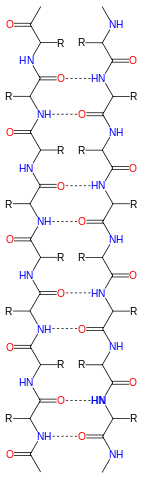
\includegraphics{antiparallel.png}
\caption{Antiparallel Folding}
\label{fig:antiparallel}
\end{center}
\end{figure}

Parallel folding is where both ends have either an N-terminus or a C-terminus.
Creates diagonal Hydrogen bonds between layers. Seen in Figure
\ref{fig:parallel}.

\begin{figure}
\begin{center}
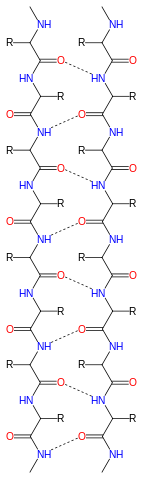
\includegraphics{parallel.png}
\caption{Parallel Folding}
\label{fig:parallel}
\end{center}
\end{figure}


\subsubsection{Amorphous Regions}

No discernable structure.


\subsection{Tertiary Structure}

Show the sequence of secondary structures that make up the protein.


\subsection{Side Chain Bonding}

Intermolecular bonding that occurs between the side chains of amino acids in
different parts of the polypeptide chain.


\subsubsection{Ionic}

One side chain has a $\ce{NH2}$ group, and another (off a different amino acid)
has a $\ce{COOH}$ group.

$\ce{COOH}$ will donate $\ce{H+}$ to $\ce{NH2}$, forming $\ce{NH3+}$ and
$\ce{COO-}$.

This forms an ionic bond between the two side chains.


\subsubsection{Hydrogen Bonds}

One side chain has a Nitrogen, Oxygen, or Fluorine atom with a lone pair of
electrons, and another has Hydrogen bonded to Nitrogen, Oxygen, or Fluorine.

Forms a Hydrogen bond between the two side chains.


\subsubsection{Dispersion Forces}

Where two side chains have very long carbon chains with a low degree of
branching.

Dispersion forces between these side chains will bond them together.


\subsubsection{Disulfide Bridge}

Where a covalent bond forms between two sulfur atoms on different side chains.




\section{Fatty Acids}

A long chain carboxylic acid commonly found in fats.


\subsection{Saturation}

Saturated fats have no double bonds in their carbon chains.

Unsaturated fats have at least one double bond.

Monounsaturated fats have 1 double bond.

Polyunsatruated fats have at least 2 double bonds.

Trans fats use the trans isomer around the double bond.




\section{Fats}

Fats are triglycerides, an ester comprised of glycerol and 3 fatty acids.


\subsection{Formation}

Formation of a triglyceride from glycerol and a fatty acid:

$$
\ce{
\chemfig{C(-[:0]OH)(-[:270]C(-[:0]OH)(-[:270]H)(-[:180]H))(-[:180]H)(-[:90]C(-[:0]OH)(-[:180]H)(-[:90]H))} +
3\chemfig{C(-[:90]H)(-[:180]H)(-[:270]H)(-[:0]C(-[:90]H)(-[:270]H)(-[:0] \,\cdots (-[:0]C(=[:45]O)(-[:-45]OH))))} ->
\chemfig{C(-[:0]O(-[:0]C(=[:90]O)(-[:0]C(-[:90]H)(-[:270]H)(-[:0]C(-[:90]H)(-[:270]H)(-[:0] \,\cdots (-[:0]C(-[:0]H)(-[:90]H)(-[:270]H)))))))
(-[:270,3]C(-[:0]O(-[:0]C(=[:90]O)(-[:0]C(-[:90]H)(-[:270]H)(-[:0]C(-[:90]H)(-[:270]H)(-[:0] \,\cdots (-[:0]C(-[:0]H)(-[:90]H)(-[:270]H)))))))
(-[:270]H)(-[:180]H))(-[:180]H)(-[:90,3]C(-[:0]O(-[:0]C(=[:90]O)(-[:0]C(-[:90]H)(-[:270]H)(-[:0]C(-[:90]H)(-[:270]H)(-[:0] \,\cdots (-[:0]C(-[:0]H)(-[:90]H)(-[:270]H)))))))(-[:180]H)(-[:90]H))} + 3H2O
}
$$



\section{Soaps}

Soap is the sodium or potassium salt of a fatty acid.


\subsection{Saponification}

Formation process called saponification.

Formed through the hydrolysis of triglycerides found in fats with a strong base
(either $\ce{NaOH}$ or $\ce{KOH}$).

Produces glycerol and the sodium or potassium salt of the fatty acid.

The salt of the fatty acid is a solid and will precipitate out of the solution.
It is collected by filtration and used as soap.

$$
\ce{
\chemfig{C(-[:0]O(-[:0]C(=[:90]O)(-[:0]C(-[:90]H)(-[:270]H)(-[:0]C(-[:90]H)(-[:270]H)(-[:0] \,\cdots (-[:0]C(-[:0]H)(-[:90]H)(-[:270]H)))))))
(-[:270,3]C(-[:0]O(-[:0]C(=[:90]O)(-[:0]C(-[:90]H)(-[:270]H)(-[:0]C(-[:90]H)(-[:270]H)(-[:0] \,\cdots (-[:0]C(-[:0]H)(-[:90]H)(-[:270]H)))))))
(-[:270]H)(-[:180]H))(-[:180]H)(-[:90,3]C(-[:0]O(-[:0]C(=[:90]O)(-[:0]C(-[:90]H)(-[:270]H)(-[:0]C(-[:90]H)(-[:270]H)(-[:0] \,\cdots (-[:0]C(-[:0]H)(-[:90]H)(-[:270]H)))))))(-[:180]H)(-[:90]H))} + 3OH- ->
3\chemfig{C(-[:90]H)(-[:180]H)(-[:270]H)(-[:0]C(-[:90]H)(-[:270]H)(-[:0] \,\cdots (-[:0]C(=[:45]O)(-[:-45]O^{-}))))} +
\chemfig{C(-[:0]OH)(-[:270]C(-[:0]OH)(-[:270]H)(-[:180]H))(-[:180]H)(-[:90]C(-[:0]OH)(-[:180]H)(-[:90]H))}
}
$$


\subsection{Emulsification}

Soaps acts as an emulsifying agent. Allows a substance that normally doesn't
dissolve in a solvent to dissolve.

Soap allows fats and oils to dissolve in water:

\begin{itemize}
\item Fatty acid has a long non-polar tail that is soluble in fats due to
	strong dispersion forces.
\item Has a polar head that is soluble in water as it is capable of forming
	Hydrogen bonds.
\item Tail embeds itself in small droplets of fat, polar heads surround the
	droplet.
\item Allows it to dissolve in water.
\end{itemize}


\subsection{Scum}

Hard water areas (like Perth) have $\ce{Ca^2+}$ and $\ce{Mg^2+}$ ions in the
water.

These form a solid precipitate with the ion of the fatty acid used in a soap.

Leaves a white residue on surfaces cleaned using the soap.

Can be prevented by softening the water using an ion exchange resin to remove
the $\ce{Ca^2+}$ and $\ce{Mg^2+}$ ions.




\section{Detergents}

Sulfonate group ($\ce{SO3-}$) used in place of carboxylic acid group:

\begin{center}
\chemfig{C(-[:90]H)(-[:180]H)(-[:270]H)(-[:0]C(-[:90]H)(-[:270]H)(-[:0] \,\cdots (-[:0]S(=[:90]O)(=[:270]O)(-[:0]O^{-}))))}
\end{center}

Doesn't form scum in hard water areas.


\subsection{Formation}

Add a long chain hydrocarbon to concentrated $\ce{H2SO4}$:

$$
\ce{
\chemfig{C(-[:90]H)(-[:180]H)(-[:270]H)(-[:0]C(-[:90]H)(-[:270]H)(-[:0] \,\cdots (-[:0]C(-[:90]H)(-[:0]H)(-[:270]H))))} + H2SO4 ->
\chemfig{C(-[:90]H)(-[:180]H)(-[:270]H)(-[:0]C(-[:90]H)(-[:270]H)(-[:0] \,\cdots (-[:0]S(=[:90]O)(=[:270]O)(-[:0]OH))))}
}
$$

Add the resulting organic product to either $\ce{NaOH}$ or $\ce{KOH}$:

$$
\ce{
\chemfig{C(-[:90]H)(-[:180]H)(-[:270]H)(-[:0]C(-[:90]H)(-[:270]H)(-[:0] \,\cdots (-[:0]S(=[:90]O)(=[:270]O)(-[:0]OH))))} + OH- ->
\chemfig{C(-[:90]H)(-[:180]H)(-[:270]H)(-[:0]C(-[:90]H)(-[:270]H)(-[:0] \,\cdots (-[:0]S(=[:90]O)(=[:270]O)(-[:0]O^{-}))))} + H2O
}
$$




\section{Biodiesel}

An organic, combustible substitute for diesel fuel.

Formed through a transesterification reaction.


\subsection{Base Catalysed Reaction}

React a triglyceride with an excess of methanol in the presence of a base:

$$
\ce{
\chemfig{C(-[:0]O(-[:0]C(=[:90]O)(-[:0]C(-[:90]H)(-[:270]H)(-[:0]C(-[:90]H)(-[:270]H)(-[:0] \,\cdots (-[:0]C(-[:0]H)(-[:90]H)(-[:270]H)))))))
(-[:270,3]C(-[:0]O(-[:0]C(=[:90]O)(-[:0]C(-[:90]H)(-[:270]H)(-[:0]C(-[:90]H)(-[:270]H)(-[:0] \,\cdots (-[:0]C(-[:0]H)(-[:90]H)(-[:270]H)))))))
(-[:270]H)(-[:180]H))(-[:180]H)(-[:90,3]C(-[:0]O(-[:0]C(=[:90]O)(-[:0]C(-[:90]H)(-[:270]H)(-[:0]C(-[:90]H)(-[:270]H)(-[:0] \,\cdots (-[:0]C(-[:0]H)(-[:90]H)(-[:270]H)))))))(-[:180]H)(-[:90]H))} +
3\chemfig{C(-[::0]OH)(-[::90]H)(-[::180]H)(-[::270]H)} <=>[OH-]
3\chemfig{C(-[:90]H)(-[:180]H)(-[:270]H)(-[:0]C(-[:90]H)(-[:270]H)(-[:0] \,\cdots (-[:0]C(=[:45]O)(-[:-45]O(-[:0]C)))))} +
\chemfig{C(-[:0]OH)(-[:270]C(-[:0]OH)(-[:270]H)(-[:180]H))(-[:180]H)(-[:90]C(-[:0]OH)(-[:180]H)(-[:90]H))} +
}
$$

Forms glycerol and 3 esters, which are the biodiesel.

The triglyceride (an ester) swaps its alcohol component with the methanol.

The glycerol must be removed as it is harmful to the engine. It forms a
separate layer on top of the biodiesel since it is insoluble in it.


\subsection{Lipase Catalysed Reaction}

React a triglyceride with an excess of methyl ethanoate in the presence of
lipase (an enzyme):

$$
\ce{
\chemfig{C(-[:0]O(-[:0]C(=[:90]O)(-[:0]C(-[:90]H)(-[:270]H)(-[:0]C(-[:90]H)(-[:270]H)(-[:0] \,\cdots (-[:0]C(-[:0]H)(-[:90]H)(-[:270]H)))))))
(-[:270,3]C(-[:0]O(-[:0]C(=[:90]O)(-[:0]C(-[:90]H)(-[:270]H)(-[:0]C(-[:90]H)(-[:270]H)(-[:0] \,\cdots (-[:0]C(-[:0]H)(-[:90]H)(-[:270]H)))))))
(-[:270]H)(-[:180]H))(-[:180]H)(-[:90,3]C(-[:0]O(-[:0]C(=[:90]O)(-[:0]C(-[:90]H)(-[:270]H)(-[:0]C(-[:90]H)(-[:270]H)(-[:0] \,\cdots (-[:0]C(-[:0]H)(-[:90]H)(-[:270]H)))))))(-[:180]H)(-[:90]H))} +
\chemfig{C(-[::0]O(-[::-45]C(=[:-135]O)(-[:0]C(-[::0]H)(-[::90]H)(-[::270]H))))(-[::90]H)(-[::180]H)(-[::270]H)} <=>[\text{lipase}]
3\chemfig{C(-[:90]H)(-[:180]H)(-[:270]H)(-[:0]C(-[:90]H)(-[:270]H)(-[:0] \,\cdots (-[:0]C(=[:45]O)(-[:-45]O(-[:0]C)))))} +
\chemfig{C(-[:0]O(-[:0]C(=[:90]O)(-[:0]C(-[:0]H)(-[:90]H)(-[:270]H))))(-[:270]C(-[:0]O-[:0]C(=[:90]O)(-[:0]C(-[:0]H)(-[:90]H)(-[:270]H)))(-[:270]H)(-[:180]H))(-[:180]H)(-[:90]C(-[:0]O-[:0]C(=[:90]O)(-[:0]C(-[:0]H)(-[:90]H)(-[:270]H)))(-[:180]H)(-[:90]H))} +
}
$$

Forms glycerol triacetate and 3 esters.

The glycerol triacetate does not harm the engine and can be burnt alongisde the
3 esters.

Methyl ethanoate is used instead of methanol as methanol denatures the lipase.

Adding an excess of methanol or methanoic acid shifts the equilibrium far right
to give a large yield of biodiesel.




\section{Sample Questions}

\subsection{Question 1}

Explain why the solubility of hydrocarbons decreases as the carbon chain length
increases.

\subsection{Question 2}

Explain why pentan-1-ol has a higher boiling point than 2-methyl butan-1-ol.

\begin{itemize}
\item Mention surface area!
\end{itemize}

\subsection{Question 3}

Explain why amines have a lower boiling point than alcohols.

\end{document}
